%%%%%%%%%%%%%%%%%%%%%%%%%%%%%%%%%%%%%%%%%
% Journal Article
% LaTeX Template
% Version 1.4 (15/5/16)
%
% This template has been downloaded from:
% http://www.LaTeXTemplates.com
%
% Original author:
% Frits Wenneker (http://www.howtotex.com) with extensive modifications by
% Vel (vel@LaTeXTemplates.com)
%
% License:
% CC BY-NC-SA 3.0 (http://creativecommons.org/licenses/by-nc-sa/3.0/)
%
%%%%%%%%%%%%%%%%%%%%%%%%%%%%%%%%%%%%%%%%%

%----------------------------------------------------------------------------------------
%	PACKAGES AND OTHER DOCUMENT CONFIGURATIONS
%----------------------------------------------------------------------------------------

\documentclass[twoside,twocolumn]{article}

\usepackage{blindtext} % Package to generate dummy text throughout this template 

\usepackage[sc]{mathpazo} % Use the Palatino font
\usepackage[T1]{fontenc} % Use 8-bit encoding that has 256 glyphs
\linespread{1.05} % Line spacing - Palatino needs more space between lines
\usepackage{microtype} % Slightly tweak font spacing for aesthetics

\usepackage[english]{babel} % Language hyphenation and typographical rules

\usepackage[hmarginratio=1:1,top=32mm,columnsep=20pt,a4paper,total={6in,9in}]{geometry} % Document margins
\usepackage[hang, small,labelfont=bf,up,textfont=it,up]{caption} % Custom captions under/above floats in tables or figures
\usepackage{booktabs} % Horizontal rules in tables

\usepackage{lettrine} % The lettrine is the first enlarged letter at the beginning of the text

\usepackage{enumitem} % Customized lists
\setlist[itemize]{noitemsep} % Make itemize lists more compact

\usepackage{abstract} % Allows abstract customization
\renewcommand{\abstractnamefont}{\normalfont\bfseries} % Set the "Abstract" text to bold
\renewcommand{\abstracttextfont}{\normalfont\small\itshape} % Set the abstract itself to small italic text

\usepackage{titlesec} % Allows customization of titles
\renewcommand\thesection{\Roman{section}} % Roman numerals for the sections
\renewcommand\thesubsection{\roman{subsection}} % roman numerals for subsections
\titleformat{\section}[block]{\large\scshape\centering}{\thesection.}{1em}{} % Change the look of the section titles
\titleformat{\subsection}[block]{\large}{\thesubsection.}{1em}{} % Change the look of the section titles

\usepackage{fancyhdr} % Headers and footers
\pagestyle{fancy} % All pages have headers and footers
\fancyhead{} % Blank out the default header
\fancyfoot{} % Blank out the default footer
\fancyhead[C]{Running title $\bullet$ May 2016 $\bullet$ Vol. XXI, No. 1} % Custom header text
\fancyfoot[RO,LE]{\thepage} % Custom footer text

\usepackage{titling} % Customizing the title section

\usepackage{hyperref} % For hyperlinks in the PDF
\usepackage{graphicx}
\graphicspath{{./img/}}
%----------------------------------------------------------------------------------------
%	TITLE SECTION
%----------------------------------------------------------------------------------------

\setlength{\droptitle}{-4\baselineskip} % Move the title up

\pretitle{\begin{center}\Huge\bfseries} % Article title formatting
\posttitle{\end{center}} % Article title closing formatting
\title{A parallelised and distributed approach to implementing Conway's Game of Life} % Article title
\author{%
\textsc{Aaron Chan}\\[1ex] % Your name
\normalsize University of Bristol \\ % Your institution
\normalsize {ho21739@bristol.ac.uk} % Your email address
\and % Uncomment if 2 authors are required, duplicate these 4 lines if more
\textsc{Ferdinand Hubbard}\\[1ex] % Second author's name
\normalsize University of Bristol \\ % Your institution
\normalsize {ej21378@bristol.ac.uk} % Your email address
}
\date{\today} % Leave empty to omit a date
\renewcommand{\maketitlehookd}{
\begin{abstract}
  We intend to explain our two solutions for implementing Conway's Game of Life in Golang, namely the Parallel and Distributed versions.
  Within this report, we will discuss the impacts of thread usage in both our implementations, as well as the effect of distributed computation as opposed to single-machine computation. In essence, we found that execution time was sped up as we increased thread count, reduced branch instructions and implemented a halo exchange mechanism.
\end{abstract}
}

%----------------------------------------------------------------------------------------

\begin{document}

% Print the title
\maketitle

%----------------------------------------------------------------------------------------
%	ARTICLE CONTENTS
%----------------------------------------------------------------------------------------
\section{Introduction to the parallel solution}

As an initial attempt, we began by implementing a 
single-threaded Game of Life (GoL) Engine, expanding upon this work 
with parallelisation by virtue of concurrent go-routine workers. 
Recognising that there exists various methods to calculating the perimeter
for \texttt{getNeighbourCount}, we tried various counting methods - taking into 
account the wrap-around feature of Game of Life.

% \begin{itemize}
%   \item single threaded implementation
%   \item events passing (alive cells, turn completed)
%   \item PGM image output implementation
%   \item SDL implementation (flipped cells events)
%   \item using channels and goroutines to create multiple workers (parallelising the solution)
%   \item switching to a memory sharing solution instead of using channels (TODO?)
%   \item implementing halo exchange
% \end{itemize}
%------------------------------------------------

\section{benchmarking methodology}
Our means of evaluating parallelisation performance gains 
was via the Go testing framework. Using 512px x 512px PGM images, we 
repeated each benchmark 10 times, taking the average runtime for each thread to acquire the central value, 
and plotting them. Each feature implementation was benchmarked in the same fashion.
% \lettrine[nindent=0em,lines=3]{L} orem ipsum dolor sit amet, consectetur adipiscing elit.
% \begin{itemize}
%   \item use built in golang benchmark framework
%   \item run command ....
%   \item output to txt
%   \item run python script to plot graphs
%   \item barchart of time taken against threads used
%   \item runs benchmarks on all pgm images
%   \item repeats benchmarks until results fall within a certain standard deviation (TBC)
% \end{itemize}
%------------------------------------------------
\begin{figure}
  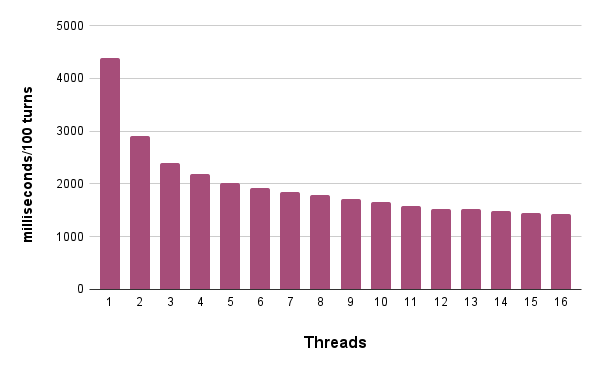
\includegraphics[width=\linewidth]{modulo.png}
  \caption{Modulo Implementation}
  \label{fig:chart1}
\end{figure}

\section{parallelising the program}
The baseline implementation's distributor function starts with
reading the image into 2D slice via \textit{io} commands, before evenly dividing 
the workload between workers. With the aid of go-routines, workers have access to the old slice
as well as the boundaries in which to process. By using \texttt{getNeighbourCount}, we apply the Game of Life
laws onto the world, piping results into a blank slice of size: \[( endRow - startRow ) \times ImageWidth\]
Sending the results back to the distributor, we integrate back together the new slices, move the pointer to the old world
to this newly-merged world and send the appropriate signals on the \textit{events}, \textit{io} channels.

\begin{figure}
  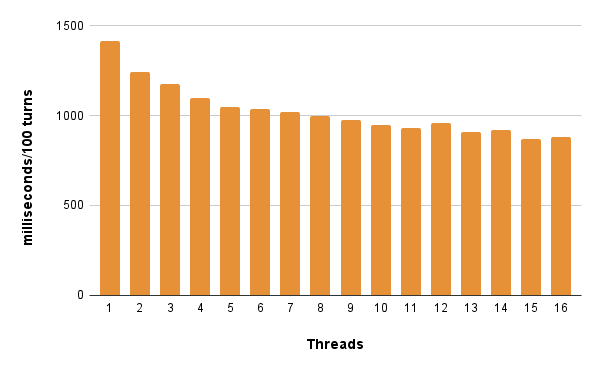
\includegraphics[width=\linewidth]{branching.png}
  \caption{Branching Implementation}
  \label{fig:chart2}
\end{figure}
\begin{figure}
  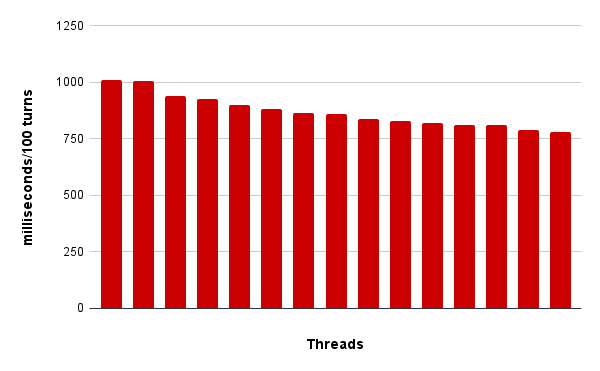
\includegraphics[width=\linewidth]{bitmask.png}
  \caption{Bitmask Implementation}
  \label{fig:chart3}
\end{figure}
% \lettrine[nindent=0em,lines=3]{L} orem ipsum dolor sit amet, consectetur adipiscing elit.
\begin{itemize}
  \item show workers pseudocode
  \item show handler pseudocode
  \item flowchart/ diagram of how channel communication workers
  \item simple flowchart of how the whole program works currently
\end{itemize}
%------------------------------------------------

\section{On the topic of analysis}

From Fig. 1, we can conclude that multithreading have an overall improvement on performance.
Statistically-speaking, we find the solution using 
modulo operations is most affected by thread usage, having standard deviation 413ms, as opposed to 107ms 
and 73ms for branching and bitmasking respectively. Interested persons will find our results achieved by:
\[SD(\forall x \in runtime : max(runtime) - x)\]
This, however, implies not that higher threads means greater 
performance as there exists other, non-parallelisable tasks, such as reading 
PGM images set a base level of execution time. 
% \lettrine[nindent=0em,lines=3]{L} orem ipsum dolor sit amet, consectetur adipiscing elit.
\begin{itemize}
  \item show graph for 5120x5120.gpm for single implementation vs parralel implementation
  \item describe the differences between each graph
  \item explain the differences by referencing the flowchart/ how the code worker
  \item explain the shape of the graph (why it resembles a 1/x graph). e.g. bottlenecks in channel communication...
\end{itemize}
%------------------------------------------------

\section{memory sharing}

% \lettrine[nindent=0em,lines=3]{L} orem ipsum dolor sit amet, consectetur adipiscing elit.
THIS SECTION WILL BE USED IF WE DECIDE TO IMPLEMENT MEMORY SHARING OVER CHANNEL COMMUNICATION
%------------------------------------------------

\section{benchmarking and critical analysis of the memory sharing}

Lorem ipsum dolor sit amet, consectetur adipiscing elit.
\blindtext % Dummy text

%------------------------------------------------

\section{Implementing Halo Exchange}

% \lettrine[nindent=0em,lines=3]{L} orem ipsum dolor sit amet, consectetur adipiscing elit.
TO BE IMPLEMENTED
%------------------------------------------------

\section{benchmarking and critical analysis of the Halo Exchange}

\lettrine[nindent=0em,lines=3]{L} orem ipsum dolor sit amet, consectetur adipiscing elit.
TO BE IMPLEMENTED
%------------------------------------------------

\section{benchmarking and critical analysis of enabling SDL}

% \lettrine[nindent=0em,lines=3]{L} orem ipsum dolor sit amet, consectetur adipiscing elit.
\begin{itemize}
  \item show graphs and describe shape and differences of with vs without SDL
  \item explain how SDL works
  \item explain how this causes bottlenecks
\end{itemize}
%------------------------------------------------

\section{comparing the parralel benchmarks}

Maecenas sed ultricies felis. Sed imperdiet dictum arcu a egestas. 
\begin{itemize}
\item Donec dolor arcu, rutrum id molestie in, viverra sed diam
\item Curabitur feugiat
\item turpis sed auctor facilisis
\item arcu eros accumsan lorem, at posuere mi diam sit amet tortor
\item Fusce fermentum, mi sit amet euismod rutrum
\item sem lorem molestie diam, iaculis aliquet sapien tortor non nisi
\item Pellentesque bibendum pretium aliquet
\end{itemize}
\blindtext % Dummy text

Text requiring further explanation\footnote{Example footnote}.

%------------------------------------------------

\section{Results}

\begin{table}
\caption{Example table}
\centering
\begin{tabular}{llr}
\toprule
\multicolumn{2}{c}{Name} \\
\cmidrule(r){1-2}
First name & Last Name & Grade \\
\midrule
John & Doe & $7.5$ \\
Richard & Miles & $2$ \\
\bottomrule
\end{tabular}
\end{table}

\blindtext % Dummy text

\begin{equation}
\label{eq:emc}
e = mc^2
\end{equation}

\blindtext % Dummy text

%------------------------------------------------

\section{Discussion}

\subsection{Areas for improvement}

A statement requiring citation \cite{Figueredo:2009dg}.
\blindtext % Dummy text

\subsection{Thanks}

\blindtext % Dummy text

%----------------------------------------------------------------------------------------
%	REFERENCE LIST
%----------------------------------------------------------------------------------------

\begin{thebibliography}{99} % Bibliography - this is intentionally simple in this template

\bibitem[Figueredo and Wolf, 2009]{Figueredo:2009dg}
Figueredo, A.~J. and Wolf, P. S.~A. (2009).
\newblock Assortative pairing and life history strategy - a cross-cultural
  study.
\newblock {\em Human Nature}, 20:317--330.
 
\end{thebibliography}

%----------------------------------------------------------------------------------------

\end{document}